\documentclass[a4paper, 10pt, spanish]{article}

\usepackage[paper=a4paper, left=1.5cm, right=1.5cm, bottom=1.5cm, top=3.5cm]{geometry}
\usepackage[spanish, es-noshorthands]{babel}
\usepackage[utf8x]{inputenc}
\usepackage[none]{hyphenat}
\usepackage[colorlinks,citecolor=black,filecolor=black,linkcolor=black,    urlcolor=black]{hyperref}

% Simbolos matemáticos
\usepackage{amsthm}
\usepackage{amsmath}
\usepackage{amsfonts}
\usepackage{amssymb}
\usepackage{algorithm}
\usepackage[noend]{algpseudocode}
\usepackage{algorithmicx}
\usepackage{listings}

% Descoración y gráficos
\usepackage{caratulaV}
\usepackage{graphicx} 
\usepackage{fancyhdr}
\usepackage{lastpage}
\usepackage{caption}
\usepackage{subcaption}
\usepackage{multirow}
\usepackage{alltt}
\usepackage{tikz}
\usepackage{varwidth,xcolor}
\usepackage{color}
\usepackage{gnuplottex}
\usepackage{verbatim}
\usepackage{framed}


% Del enunciado
\usepackage{a4wide}
\usepackage{amsmath}
\usepackage{amsfonts}
%\usepackage[ruled,vlined]{algorithm2e}

\newcommand{\kknn}{k}
\newcommand{\kpca}{\alpha}
\newcommand{\kkfold}{K}

% Acomodo fancyhdr.
\pagestyle{fancy}
\thispagestyle{fancy}
\addtolength{\headheight}{1pt}
\lhead{Algoritmos y estructuras de datos III}
\rhead{$2^{\mathrm{do}}$ cuatrimestre de 2015}
\cfoot{\thepage /\pageref*{LastPage}}
\renewcommand{\footrulewidth}{0.4pt}

\floatname{algorithm}{Pseudocodigo}
\algrenewcommand\algorithmicfunction{\textbf{Funcion}}
\algrenewcommand\algorithmicwhile{\textbf{mientras}}
\algrenewcommand\algorithmicfor{\textbf{para}}
\algrenewcommand\algorithmicforall{\textbf{para cada}}
\algrenewcommand\algorithmicdo{\textbf{hacer:}}
\algrenewcommand\algorithmicif{\textbf{si}}
\algrenewcommand\algorithmicthen{\textbf{entonces:}}
\algrenewcommand\algorithmicelse{\textbf{si no:}}
\algrenewcommand\algorithmicend{\textbf{fin}}
\algrenewcommand\algorithmicreturn{\textbf{devolver}}



\sloppy

\parskip=5pt % 10pt es el tama de fuente

% Pongo en 0 la distancia extra entre itemes.
\let\olditemize\itemize
\def\itemize{\olditemize\itemsep=0pt}



\usepackage{tikz}
%\usepackage{tikz-qtree}


\usetikzlibrary{arrows,backgrounds,calc}

\pgfdeclarelayer{background}
\pgfsetlayers{background,main}

\newcommand{\real}{\mathbb{R}}
\newcommand{\nat}{\mathbb{N}}

\newcommand{\revJ}[1]{{\color{red} #1}}

\newcommand{\convexpath}[2]{
[ 
    create hullnodes/.code={
        \global\edef\namelist{#1}
        \foreach [count=\counter] \nodename in \namelist {
            \global\edef\numberofnodes{\counter}
            \node at (\nodename) [draw=none,name=hullnode\counter] {};
        }
        \node at (hullnode\numberofnodes) [name=hullnode0,draw=none] {};
        \pgfmathtruncatemacro\lastnumber{\numberofnodes+1}
        \node at (hullnode1) [name=hullnode\lastnumber,draw=none] {};
    },
    create hullnodes
]
($(hullnode1)!#2!-90:(hullnode0)$)
\foreach [
    evaluate=\currentnode as \previousnode using \currentnode-1,
    evaluate=\currentnode as \nextnode using \currentnode+1
    ] \currentnode in {1,...,\numberofnodes} {
-- ($(hullnode\currentnode)!#2!-90:(hullnode\previousnode)$)
  let \p1 = ($(hullnode\currentnode)!#2!-90:(hullnode\previousnode) - (hullnode\currentnode)$),
    \n1 = {atan2(\x1,\y1)},
    \p2 = ($(hullnode\currentnode)!#2!90:(hullnode\nextnode) - (hullnode\currentnode)$),
    \n2 = {atan2(\x2,\y2)},
    \n{delta} = {-Mod(\n1-\n2,360)}
  in 
    {arc [start angle=\n1, delta angle=\n{delta}, radius=#2]}
}
-- cycle
}

\newcommand{\todo}[1]{
\textbf{\color{red}{\underline{Nota:} #1}}
}

\newcommand\param[3]{\ensuremath{\mathbf{\textbf{#1}}\,#2\!:} \texttt{#3}}

\let\state\State
\let\while\While
\let\endwhile\EndWhile
\let\endif\EndIf
\let\elseif\ElsIf
\let\for\For
\let\endfor\EndFor
\let\function\Function
\let\endfunction\EndFunction


\newcommand{\degree}{\ensuremath{^\circ}}

\begin{document}
%\setcounter{tocdepth}{2}
\renewcommand{\tablename}{Tabla} 


\thispagestyle{empty}
\materia{Algoritmos y estructuras de datos III}
\submateria{Segundo Cuatrimestre de 2015}
\titulo{Trabajo Práctico II}

\integrante{Federico De Rocco }{403/13}{fede.183@hotmail.com}
\integrante{Federico Nicolás Esquivel}{915/12}{alt.juss@gmail.com}

\maketitle
\newpage
%\begin{titlepage}

%\maketitle

%\end{titlepage}
\setcounter{page}{1}

\newpage
\tableofcontents

\newpage


\newpage


\section{Ejercicio 1}
\subsection{Introducción}
El problema consiste en hallar el camino que utilice la mayor cantidad posible de portales para llegar desde el piso 0 al N.
En este contexto, los portales solo llevan a pisos superiores, nunca bajan.
Se garantiza que existe un camino m\'aximo entre los pisos mencionados y que no hay m\'as de un portal que comunique el mismo par de pisos.

\subsection{Desarrollo}
A fin de encontrar el camino mas largo en tiempo cuadrático sobre la cantidad de pisos, planteamos una solución con programación dinámica.
Podemos definir recursivamente el largo del camino con la máxima cantidad de portales atravesados para llegar a un piso dado hasta el piso n como:

\begin{center}
$P_N(p) =max_{p' \in suc(p)}\{ 1 + P_N(p')\}$
\end{center}

Donde $suc(p)$ son los pisos que tienen un portal con origen en $p$.

Implementamos este comportamiento con una representación como listas de antecesores.

Partimos desde el último piso, indicándolo como accesible, e iteramos hacia abajo. 
Para cada piso, si es accesible desde el piso N, por cada antecesor calculamos el máximo entre el valor ya calculado (si lo hay) 
y la cantidad de portales hasta el enésimo piso sumado uno, y memorizamos este resultado. Podría existir un valor previo si el antecesor en cuestión también lo es para algún piso superior.
Hecho esto, marcamos sus antecesores como accesibles y continuamos iterando hasta llegar al piso 0.

Cuando esto suceda, como sabemos que existe camino entre último piso y la planta baja, habremos calculado $P_N(0)$.

Implementamos este comportamiento con el siguiente algoritmo:

\begin{algorithm}
\caption{Camino Máximo}\label{alg-ej1}
\begin{algorithmic}[1]
\Procedure{CaminoMáximo}{}
\State $\textit{pisos} \gets \text{lista de antecesores}$
\State $\textit{accesible} \gets \text{arreglo de tamaño }N$
\State $\textit{maximoDesdeN} \gets \text{arreglo de tamaño }N$
\State Inicializar $accesible$ en 0 para todas sus posiciones
\State Inicializar $maximoDesdeN$ en 0 para todas sus posiciones
\State $accesible_N \gets true $ 

\for {$p = N\text{ hasta }0$}
\State $piso \gets pisos_i$
\If {$\textit{accesible}_p$}
\for{$antecesor$ en $piso.antecesores$}
\State $maximo \gets\max\{maximoDesdeN_{piso.numero} + 1 , maximoDesdeN_{antecesor}\}$
\State $maximoDesdeN_{antecesor} \gets maximo$
\State $accesible_{antecesor} \gets true$
\EndFor
\EndIf
\EndFor  
\Return $maximoDesdeN_{0}$
\EndProcedure
\end{algorithmic}
\end{algorithm}

En el código utilizamos una estructura propia para representar cada piso, que agrupa el número de piso y una lista de los números de los antecesores. Ésta lista se implementa como una lista enlazada, por lo que tiene costo de inserción constante. En el algoritmo descrito, $pisos$ es una arreglo de estas estructuras, ordenada por numero de piso cuando es construida. Esto tiene lugar de la siguiente manera: 

\begin{algorithm}
\caption{Inicialización Camino Máximo}\label{init-ej1}
\begin{algorithmic}[2]
\Procedure{Init}{}
\State $\textit{pisos} \gets \text{arreglo de tamaño }N$

\for {$i = 0\text{ hasta }N$}
\State $antecesores \gets \text{nueva Lista de }int$
\State $piso \gets \text{nuevo }\textit{Piso(i,antecesores) }$
\State $pisos_i \gets piso $
\EndFor  

\for{$portal$ en $portales$}
\State $pisos_{portal.hasta}.antecesores.agregarAtras( portal.desde )$
\EndFor

\EndProcedure
\end{algorithmic}
\end{algorithm}



\subsection{Correctitud}

Como iteramos desde el piso N al 0, partiendo de $P_N(N) = 0$, cuando estemos iterando sobre el piso $p$, si hay portales que lo conecten con el último piso, ya tendremos $P_N(p)$ correctamente calculado y memorizado.
Podemos afirmar esto porque como los portales solo suben, el piso $p$ no puede ser antecesor de ningún piso sobre el cual nos falte iterar, pues como puede verse en el algoritmo \ref{alg-ej1}, $maximoDesdeN$ (el vector donde memorizamos los resultados de $P_N$) solo se modifica en las posiciones correspondientes a antecesores del piso sobre el cual se itera.

Por lo tanto, ya habremos calculado $P_N(p_s)$ para todos los sucesores $p_s$ del piso $p$ y memorizado el máximo entre ellos. 

Una vez que la iteración sobre los pisos termina, sea $l = P_N(p)$ el largo de la ruta desde el piso $p$ al $N$, supongamos que no es máxima.
Si esto sucede, hay un camino desde este piso al último que usa al menos un portal más.  Entonces existe $p'$ sucesor de $p$, tal que $P_N(p') \geq l$. 

Por otro lado $l$ es el máximo de todos los caminos entre los sucesores de $p$ y $N$, sumado uno, por lo que podemos decir que $l > P_N(p_s)$ para todo $p_s$ sucesor de $p$.
En particular, al ser sucesor de $p$, $l > P_N(p')$, lo que lleva a $l > P_N(p') \geq l$. Luego, esta suposición es absurda.

\subsection{Complejidad}

Como no hay portales de un piso superior a uno inferior, para cada piso sus antecesores serán pisos debajo de el. Luego, para un piso $p$, sus antecesores serán a lo sumo $p-1$ pisos.

De acuerdo a lo expuesto en el algoritmo descrito en el pseudocódigo \ref{alg-ej1}, entre las lineas 8 y 14 iteramos sobre la cantidad de pisos.
Asimismo dentro de cada ejecución del ciclo, si el $\textit{p-ésimo}$ piso es accesible, repetimos las lineas 12 a 14 por cada antecesor. Es decir, estas operaciones se repiten $p-1$ veces. Cada una de estas sentencias se ejecuta en tiempo constante, ya que son comparaciones, asignaciones o accesos sobre arreglos. Por lo tanto, sumando el costo de las operaciones tenemos:
\begin{center}
$\sum_{p=1}^{N}(p-1) = \frac{1}{2}(N-1)n$
\end{center}

Luego, podemos acotar el orden de complejidad de la ejecución del algoritmo por $O(\frac{1}{2}(N-1)N)$ que es equivalente a $O(N^2)$.

Por otro lado, el costo de inicializar las estructuras requeridas por el algoritmo usando el procedimiento descrito en el pseudocódigo \ref{init-ej1} es $O(N+P)$, con $P$ la cantidad de portales.
En esta cota consideramos que el costo de inicialización del arreglo $pisos$ es $O(N)$, y crear una lista vacía y el par que la relaciona al número de piso tiene costo constante.

De igual manera, el acceso sobre el vector de pisos y la inserción sobre la lista de antecesores tienen costo $O(1)$, y al repetirse una vez por cada portal, suman $P$ a la complejidad. La cantidad de portales esta contemplada en el algoritmo como la suma de los antecesores de cada piso, que como establecimos anteriormente, es $\frac{1}{2}(N-1)N$, que podemos acotar asintóticamente por $O(N^2)$.

Finalmente, el costo de inicializar y ejecutar algoritmo se puede acotar por $O(N^2)$.








\subsection{Experimentación}

Se plantean una serie de casos de prueba para los cuales esperamos obtener resultados correctos en base a lo expuesto en las secciones anteriores.
Las primeras tres pruebas se basan en generar un camino simple en el cual
todos los nodos sean necesarios para llegar desde el primer piso al último. Los siguientes grafos son las representaciones de estos casos. El punto de partida es el nodo 1 y
el de llegada es el que tenga mayor valor.

\begin{tikzpicture}
\node(pseudo) at (-1,0){};
\node(0) at (0,0)[shape=circle,draw]        {$0$};
\node(1) at (0,2)[shape=circle,draw]        {$1$};

\path [->]
  (0)      edge                 node [above]  {}     (1);

\end{tikzpicture}

Resultado: 1

\begin{tikzpicture}
\node(pseudo) at (-1,0){};
\node(0) at (0,0)[shape=circle,draw]        {$0$};
\node(1) at (0,1)[shape=circle,draw]        {$1$};
\node(2) at (0,2)[shape=circle,draw]        {$2$};

\path [->]
  (0)      edge                 node [above]  {}     (1)
  (1)      edge                 node [above]  {}     (2);

\end{tikzpicture}

Resultado: 2

\begin{tikzpicture}
\node(pseudo) at (-1,0){};
\node(0) at (0,0)[shape=circle,draw]        {$0$};
\node(1) at (0,1)[shape=circle,draw]        {$1$};
\node(2) at (0,2)[shape=circle,draw]        {$2$};
\node(3) at (0,3)[shape=circle,draw]        {$3$};

\path [->]
  (0)      edge                 node [above]  {}     (1)
  (1)      edge                 node [above]  {}     (2)
  (2)      edge                 node [above]  {}     (3);

\end{tikzpicture}

Resultado: 3

Para el siguiente experimento buscamos observar el funcionamiento cuando existen dos caminos con el mismo largo.

\begin{tikzpicture}
\node(pseudo) at (-1,0){};
\node(0) at (2,0)[shape=circle,draw]        {$0$};
\node(1) at (0,2)[shape=circle,draw]        {$1$};
\node(2) at (0,4)[shape=circle,draw]        {$3$};
\node(3) at (2,6)[shape=circle,draw]        {$5$};
\node(4) at (4,3)[shape=circle,draw]        {$2$};
\node(5) at (4,5)[shape=circle,draw]        {$4$};

\path [->]
  (0)      edge                 node [above]  {}     (1)
  (1)      edge                 node [above]  {}     (2)
  (2)      edge                 node [above]  {}     (3)
  (0)      edge                 node [above]  {}     (4)
  (4)      edge                 node [above]  {}     (5)
  (5)      edge                 node [above]  {}     (3);
  

\end{tikzpicture}

Resultado: 3

Después repetimos lo anterior pero con la diferencia que los dos caminos son distintos en longitud.

\begin{tikzpicture}
\node(pseudo) at (-1,0){};
\node(0) at (2,0)[shape=circle,draw]        {$0$};
\node(1) at (0,1)[shape=circle,draw]        {$1$};
\node(2) at (0,2)[shape=circle,draw]        {$2$};
\node(3) at (2,9)[shape=circle,draw]        {$8$};
\node(4) at (4,3)[shape=circle,draw]        {$3$};
\node(5) at (4,5)[shape=circle,draw]        {$4$};
\node(6) at (4,6)[shape=circle,draw]        {$5$};
\node(7) at (4,7)[shape=circle,draw]        {$6$};
\node(8) at (4,8)[shape=circle,draw]        {$7$};

\path [->]
  (0)      edge                 node [above]  {}     (1)
  (1)      edge                 node [above]  {}     (2)
  (2)      edge                 node [above]  {}     (3)
  (0)      edge                 node [above]  {}     (4)
  (4)      edge                 node [above]  {}     (5)
  (5)      edge                 node [above]  {}     (6)
  (6)      edge                 node [above]  {}     (7)
  (7)      edge                 node [above]  {}     (8)
  (8)      edge                 node [above]  {}     (3);

\end{tikzpicture}

Resultado: 6 (Recorrerá el camino $0\rightarrow3\rightarrow4\rightarrow5\rightarrow6\rightarrow7\rightarrow8$ que es el más largo).

Para los siguientes experimentos lo que haremos es tener por un lado un camino corto que nos lleva del origen al destino y otro camino que nos lleve a este, pero sin comenzar
por el origen.

\begin{tikzpicture}
\node(pseudo) at (-1,0){};
\node(0) at (2,0)[shape=circle,draw]        {$0$};
\node(1) at (4,1)[shape=circle,draw]        {$1$};
\node(2) at (4,2)[shape=circle,draw]        {$2$};
\node(3) at (4,3)[shape=circle,draw]        {$3$};
\node(4) at (0,4)[shape=circle,draw]        {$4$};
\node(5) at (2,5)[shape=circle,draw]        {$5$};


\path [->]
  (0)      edge                 node [above]  {}     (4)
  (1)      edge                 node [above]  {}     (2)
  (2)      edge                 node [above]  {}     (3)
  (3)      edge                 node [above]  {}     (5)
  (4)      edge                 node [above]  {}     (5);


\end{tikzpicture}

Resultado: 2.

\begin{tikzpicture}
\node(pseudo) at (-1,0){};
\node(0) at (2,0)[shape=circle,draw]        {$0$};
\node(1) at (4,1)[shape=circle,draw]        {$1$};
\node(2) at (4,2)[shape=circle,draw]        {$2$};
\node(3) at (4,3)[shape=circle,draw]        {$3$};
\node(4) at (4,4)[shape=circle,draw]        {$4$};
\node(5) at (2,5)[shape=circle,draw]        {$5$};


\path [->]
  (0)      edge                 node [above]  {}     (5)
  (1)      edge                 node [above]  {}     (2)
  (2)      edge                 node [above]  {}     (3)
  (3)      edge                 node [above]  {}     (4);

\end{tikzpicture}

Resultado: 1.

Como podemos ver la idea es que tenga por resultado la cantidad de portales que tiene que atravesar en el camino que comienza en el origen y concluye en el destino, y no
los que no cumplan esta última propiedad.

Lo siguiente serán unos tests dedicados a la medición de tiempos. Graficaremos los casos por separado y con distintos tamaños ya que la diferencia de tiempos entre el mejor y peor caso es demasiado
grande como para ponerlos en un solo gráfico, ya que se perderían detalles.

En estas mediciones no consideramos el tiempo de incialización, que consideramos parte de la lectura de la entrada.

 Comenzemos por el peor caso el cual conseguimos mediante un grafo completo, por completo nos 
refirimos a que cada piso tiene un portal por cada uno de los siguientes. Con más posibilidades debemos que tener en cuenta todas para obtener el camino con mayor número 
de portales. Para el caso promedio simplemente nos armaremos un grafo aleatorio que partirá de la base que del caso anterior, osea que hay un camino que involucra a todos los 
nodos y agregaremos aristas entre los nodos de forma aleatoria. El tamaño de las muestra variara entre 200 y 290 con saltos de 10.

\begin{figure}[H]
\input{plots/Tp2Ej1ExpPeor.tex}
\caption{Comparación de tiempos variando la cantidad de pisos}
\end{figure}

Para el mejor caso, podríamos simplemente un grafo similar al del último test de correctitud. En otras palabras que el comienzo este unido con el fin y los nodos intermedios 
no influyan. Dado que este caso es poco interesante porque solamente hay una posibilidad y el tiempo sería constante, hemos decidido omitir este caso como trivial y asumir que el 
mejor caso a evaluar es en el cual exista un camino entre el primero y el último que pase por todos los nodos(semejante a los primeros tests de correctitud). Variaremos el 
tamaño de las muestras de 200 a 2000 con saltos de 200. Usamos esta muestra tan grande porque usando la anterior no nos permite apreciar suficiente diferencia.

\begin{figure}[H]
\input{plots/Tp2Ej1ExpMejor.tex}
\caption{Comparación de tiempos variando la cantidad de pisos}
\end{figure}




\section{Ejercicio 2}
\subsection{Introducción}
En este problema buscamos minimizar el tiempo necesario para llegar desde el principio del pasillo en la planta baja al final del pasillo en el último piso.
Se garantiza que existe al menos un camino entre estos puntos.


\subsection{Desarrollo}
Para resolver este ejercicio en la complejidad pedida consideramos usar un algoritmo Breadth-First Search.
Sin embargo, como usar un portal tiene costo distinto a caminar en el mismo piso y los portales pueden estar a cualquier distancia entre si, necesitamos primero normalizar los costos.
Para ello consideramos en lugar de un grafo con solo portales como vértices, uno donde cada posición de cada piso esta representada.
De ésta forma, entre portales del mismo piso hay tantos vértices como posiciones intermedias, y atravesar cada una tiene costo 1, por lo que es suficiente contar la cantidad vértices.
Como utilizar un portal tiene costo 2, agregamos un nodo intermedio entre las ubicaciones que comunica cada portal.
De esta forma, la distancia entre cada posición y portal queda definida por la cantidad de vértices intermedios, con lo cual podemos aplicar BFS para obtener el resultado.


Para representar esta conversión, usamos una matriz de $N+1 \times  L+1$ posiciones (incluimos desde la posición $0$ a la $L$ de cada piso), donde cada posición almacena su piso, metro, distancia hasta ella -inicialmente 0, indicando que no fue calculada- y sus vecinos. 
Para cada una, sus vecinos son los destinos de cualquier portal que este ubicado allí y las posiciones contiguas a izquierda y derecha, si existen. A partir de los parámetros de entrada $N$, $L$ y la lista de portales, se construye esta matriz de acuerdo al siguiente procedimiento:


\begin{algorithm}[H]
\caption{Inicialización de Camino Mínimo}\label{init-ej2}
\begin{algorithmic}[3]
\Procedure{Init}{}
\State $\textit{N} \gets \text{cantidad de pisos}$
\State $\textit{L} \gets \text{largo de pasillos}$
\State $\textit{portales} \gets \text{lista de portales}$
\State $mapaPortales \gets $matriz de $N+1$ filas y $L+1$ columnas

\for {$i = 0\text{ hasta }N$}
\for{$j = 0\text{ hasta }L$}
\State $vecinos \gets \text{nueva lista vacía de}Posicion$
\State $pos \gets \text{nueva }Posicion(i,j,vecinos) $
\State $mapaPortales_{i,j} \gets pos$
\EndFor
\EndFor

\for {$i = 0\text{ hasta }N$}
\for{$j = 0\text{ hasta }L$}
\If{$j > 0$}
\State $mapaPortales_{i,j}.vecinos.agregarAtras(mapaPortales_{i,j-1})$
\EndIf
\If{$j < l$}
\State $mapaPortales_{i,j}.vecinos.agregarAtras(mapaPortales_{i,j+1})$
\EndIf
\EndFor
\EndFor


\for {cada $portal$ en $portales$}
\State $d \gets portal.desde$
\State $h \gets portal.hasta$
\State $mapaPortales_{d.piso, d.metros}.vecinos.agregarAtras(mapaPortales_{h.piso, h.metros})$
\State $mapaPortales_{h.piso, h.metros}.vecinos.agregarAtras(mapaPortales_{d.piso, d.metros})$
\EndFor
  

\EndProcedure
\end{algorithmic}
\end{algorithm}


Mientras calculamos distancias entendemos que hay un portal entre una posición y su vecino si están en diferentes pisos, o a mas de un metro de distancia en el mismo piso. 
Si hubiera un portal entre dos ubicaciones contiguas no lo consideramos, dado que es más barato caminar entre ellas.
Cuando existe un portal, encolamos el vértice intermedio, cuyo único vecino es el nodo destino del portal al que corresponde.\\
Se implementa este comportamiento por medio del siguiente algoritmo:



\begin{algorithm}[H]
\caption{Camino Mínimo}\label{alg-ej2}
\begin{algorithmic}[4]
\Procedure{CaminoMinimo}{}
\State $mapaPortales \gets$ matriz de $N$ filas y $L$ columnas construida con el procedimiento \ref{init-ej2}
\State $\textit{verticesRestantes} \gets \text{cola de }Posicion$
\State $\textit{verticesRestantes}.encolar(mapaPortales_{0,0})$

\while {$verticesRestantes$ no vacía}
\State $pos \gets verticesRestantes.desencolar()$
\for{$Posicion destino$ en $pos.vecinos$}
\If{$destino.distancia = 0$}
\If{$hayPortal(pos,destino)$}
\State $portalBuffer \gets$ nueva $Posicion(destino.piso, destino.metro)$
\State $portalBuffer.distancia = pos.distancia + 1$
\State $portalBuffer.vecinos.agregarAtras(destino)$
\State $verticesRestantes.encolar(portalBuffer)$
\Else
\State $destino.distancia = pos.distancia + 1$
\State $verticesRestantes.encolar(destino)$
\EndIf
\EndIf
\EndFor
\EndWhile

\Return $mapaPortales_{N,L}.distancia$


\EndProcedure
\end{algorithmic}
\end{algorithm}


Al terminar el algoritmo, devolvemos el costo de llegar a la última posición del último piso.




\subsection{Correctitud}

Tal como describimos en la sección anterior, representamos los costos añadiendo nodos intermedios. El costo de moverse entre dos posiciones en un piso es de un segundo por metro, es decir, igual a la cantidad de metros. 
En el algoritmo propuesto, construimos la matriz $mapaPortales$ de tamaño $N+1 \times L+1$ donde cada elemento $mapaPortales_{i,j}$ representa la posición en el piso $i$ a los $j$ metros del inicio del pasillo. 
De esta manera, todos los metros de cada pasillo están representados en la matriz. 
Adicionalmente, como se puede observar en el pseudocódigo \ref{init-ej2} (lineas 11 a 16), cada elemento tiene como vecinos a sus posiciones aledañas.

Durante la ejecución del algoritmo tomamos cada elemento de la matriz como un vértice, por lo que la distancia en metros entre dos posiciones del mismo piso resulta ser igual a la cantidad de vértices intermedios.


Análogamente, al agregar un nodo intermedio para cada portal, igualamos el costo de utilizarlos al número de vértices a recorrer para llegar a destino agregando un nodo intermedio, de acuerdo a lo expuesto en el pseudocódigo \ref{alg-ej2} (lineas 9 a 13). 

Finalmente, el algoritmo se reduce a BFS: Se encola un nodo inicial y mientras la cola no este vacía, se desencola un nodo $n$, se encolan todos sus vecinos y se le asigna a cada uno la distancia de $n$ al origen más uno, si no estaba ya calculada.
Por lo tanto, podemos asegurar que el algoritmo es correcto a partir de la correctitud de BFS, probada en la bibliografía \cite{Cormen}.


\subsection{Complejidad}

Para la inicialización de la estructura en la que se basa el algoritmo, de acuerdo a lo descrito en el pseudocódigo \ref{init-ej2}, se itera sobre las $N+1$ filas y $L+1$ columnas de la matriz para inicializarla y luego asignar los vecinos adyacentes a cada posición. Finalmente, se itera sobre la cantidad de portales para añadir las posiciones conectadas a las listas de vecinos correspondientes. La lista de vecinos se implementa sobre una lista enlazada y sus inserciones se realizan en tiempo constante. De igual manera, la construcción de instancias del tipo $Posicion$ también tiene costo $O(1)$. A partir de esto, podemos acotar el costo de inicialización por $O(NL + P)$


Dada la representación elegida, tenemos $NL + P$ vértices, uno por cada metro en cada pasillo, y uno intermedio por cada portal.
Asimismo, la cantidad de aristas por cada posición $p_{i,j}$ es $2 + Portales(p_{i,j})$, donde $i$ es el piso, $j$ el metro y $Portales(x)$ la cantidad de portales con un extremo en la posición $x$.

Como cada portal es bidireccional, se representa en ambos extremos (ver pseudo \ref{alg-ej2}, lineas 18 a 21), por lo que durante la ejecución de BFS se suma dos veces.
Luego, la cantidad de aristas del grafo es $2 (NL + P)$

Durante la ejecución del algoritmo, por cada vértice en la cola se ejecutan operaciones, que dadas las estructuras utilizadas son $O(1)$, tantas veces como vecinos tenga ese nodo.
Si el grafo es conexo, como para cada vértice se encolan sus vecinos no visitados, el ciclo se ejecuta una vez por nodo. Si no fuera conexo, se visitarán menos vértices.

Entonces, cada ejecución del ciclo principal sobre un vértice $v$ tiene un costo $O(1 + E_v)$, con $E_v$ la cantidad de aristas incidentes a $v$. Como en el peor caso (grafo conexo) se visitan todos los nodos del grafo, la sumatoria de este costo sobre todos ellos es $O(|V| + |E|)$, donde $V$ y $E$ son los conjuntos de vértices y aristas del grafo respectivamente. 

Como establecimos previamente, la cantidad de vértices del grafo que consideramos es $NL + P$, y la de aristas es $2 (NL + P)$, por lo que el costo en peor caso suma $O((NL + P) + 2(NL + P))$, que queda acotado por $O( NL + P )$.

\subsection{Experimentación}

Dado que la complejidad temporal del código de inicialización es igual al del algoritmo, decidimos obviarlo de las mediciones de tiempos y concentrar nuestro análisis en el código que resuelve el problema.

Consideramos el grafo completo como el peor caso, ya que al ser conexo se analizan todos los vertices, y cada uno tiene la máxima cantidad de vecinos. En particular, al haber un portal entre el principio del pasillo en planta baja y el final en el último piso, el resultado esperado es $2$.
Al estar dado por la máxima cantidad de portales, que depende del tamaño del grafo ya que cada posición puede tener un portal a cada una de las $NL - 1$ posiciones restantes, observamos los tiempos variando $NL$.

Para el mejor caso consideramos que al tener como única restricción la existencia de un camino entre la primer posición de la planta baja y la última de la mas alta, basta incluir un portal desde el piso $0$ al $N$. Elegimos un portal entre la posición inicial y final, con lo que el resultado esperado es el mismo al del caso anterior.
Análogamente al anterior, este caso se da en la mínima cantidad de portales, por lo que realizamos el mismo análisis en función de $NL$.

En los experimentos realizados se observaron resultados similares al fijar una variable del producto $NL$, aumentando la otra para variarlo.

\begin{figure}[H]
\input{plots/Tp2Ej2Exp1.tex}
\caption{Comparación de tiempos variando NL}
\end{figure}

Omitimos de esta figura las mediciones del mejor caso, dado que involucra $2L$ vértices, pues la componente conexa que contiene la primer posición del piso 0 y la última del piso N esta compuesta por los nodos de ambos pasillos, sus tiempos de ejecución son mucho menores a los de peor caso, aun aumentando $L$ para variar $NL$.


Como no realizamos optimizaciones sobre BFS para especializarlo al problema de la búsqueda de camino mínimo de uno a uno, el costo del algoritmo es el mismo para cualquier par de metros en los pisos elegidos, pues se analizan la misma cantidad de nodos y ejes.
Esto es porque se calcula la distancia a todos los vértices de la componente conexa del nodo original. Debido a la forma de representar el problema que elegimos, en la ausencia de portales tenemos por cada piso una componente conexa. Al agregar portales entre pisos, las unimos. 


Dado que para este algoritmo, una vez que se calcula la distancia a un nodo sabemos que su valor es final, podríamos detener la ejecución ni bien se calcule la distancia a la posición final. Para esto, agregamos al algoritmo descrito en el pseudocódigo \ref{alg-ej2} un chequeo sobre la distancia a la posición en $mapaPortales_{N,L}$ luego de calcular la distancia para cada vecino de una posición, y devolvemos ese valor si ya fue calculado.

La complejidad temporal sigue estando acotada por $O(NL+P)$, pero en ciertos casos 
mejora considerablemente el tiempo de ejecución. 

Con esta modificación, entendemos que el peor caso se dará cuando se deban visitar todos los nodos antes de llegar al vértice objetivo. Esto sucede cuando se cuenta con un grafo completo entre los pisos 0 y N-1, con el último piso conectado en su posición 0 con algún nodo del anterior.

\begin{figure}[H]
\input{plots/Tp2Ej2Exp2.tex}
\caption{Comparación de tiempos variando NL}
\end{figure}

Nuevamente omitimos de la figura el mejor caso. Con esta modificación, en ese escenario solo se calcula la distancia al vértice objetivo independientemente de la cantidad de vértices o portales, por lo que su tiempo de ejecución es casi inmediato.






\section{Ejercicio 3}
\subsection{Introducción}
Contamos con un conjunto de exploradoras a las que se le asigna una letra, cada una con amistades dentro del grupo. 
A partir de esto, buscamos ubicarlas en una ronda que minimice la suma de las distancias entre cada par de amigas.
De esa ronda queremos saber ademas cual fue la distancia máxima entre amigas, y de haber mas de una ronda posible, quedarnos con la primera en orden alfabético.\\
Se pide una complejidad estrictamente mejor que $O(e^ea^2) $, donde $e$ es la cantidad de exploradoras y $a$ la cantidad de amistades.

Por ejemplo:
\\
Se cuenta con las exploradoras  $e = \{a, b, c, d, e\} $  y amistades  $a = \{ (a,b), (a,c), (a,d), (b,e), (c,d) \} $ 

\begin{figure}[H]
  \hspace{-2em}
	\begin{minipage}[h]{0.48\textwidth}
	\begin{center}
		\centering
		  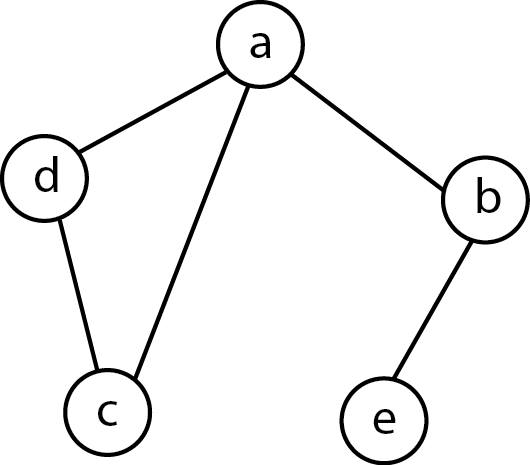
\includegraphics[scale=1]{imagenes/ej3-ejemplo.png}
		 \caption{Ejemplo de configuración óptima}
	\end{center}
	\end{minipage}
	\hspace{3em}
	\begin{minipage}[h]{0.48\textwidth}
	\begin{center}
	   \centering
	       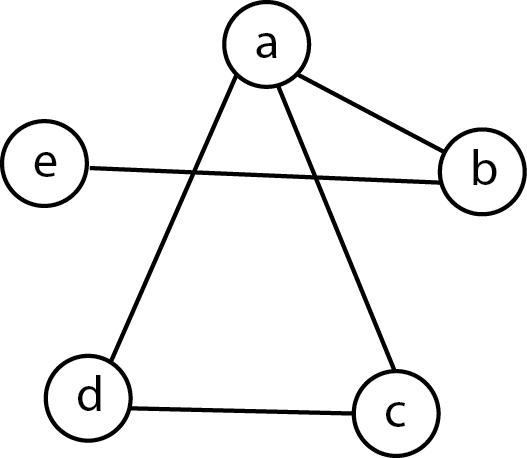
\includegraphics[scale=1]{imagenes/ej3-ejemplo2.png}
	     \caption{Ejemplo de configuración suboptima}
	\end{center}
	\end{minipage}
\end{figure}

La ronda que minimiza la suma de las distancias entre las amistades primera en orden alfabético es $abecd$, donde la distancia para cada amistad es una exploradora, excepto $(a,c)$ que tienen una separación de dos , sumando una distancia total $6$. Para el caso $abcde$, las amistades $(a,b)$ y $(c,d)$ tienen distancia uno, mientras que las demás están separadas por dos, sumando un total de $8$.


\subsection{Desarrollo}
Elegimos utilizar la técnica de backtracking para hallar una solución optima.
A partir de los datos de entrada, construimos una lista de exploradoras en la que guardamos su letra y posición en la ronda. Para indicar que una exploradora no esta en la ronda, utilizamos el indice -1.
Luego definimos una lista de amistades que vincula pares de exploradoras de la lista anterior.
Por último, ordenamos alfabéticamente la lista de exploradoras, para facilitar el orden en que buscaremos soluciones optimas.

Dado que es una estructura circular, siempre podremos ubicar la primer exploradora (por su letra) en la primer posición al representar cualquier ronda optima como una cadena. Al tener la lista de exploradoras ordenada, la primera de la lista estará en el primer lugar a imprimir, por lo que la ubicamos antes de llamar a la función de backtracking. Esto no es estrictamente necesario para la solución, pero elimina una cantidad considerable de operaciones innecesarias.

\newpage

Hecho esto, llamamos a la función recursiva que resuelve el problema.
En cada llamada calculamos primero la suma de las distancias entre las amistades presentes en la ronda. Si esta suma es menor a la mejor solución encontrada, o aun no hallamos una, y faltan exploradoras para completar la ronda, ubicamos cada exploradora posible en la posición actual y llamamos a la recursión indicando que se debe ubicar la siguiente. Si la ronda esta completa, guardamos la suma si es mejor que nuestra solución anterior. Si la suma parcial fue mayor a nuestro candidato a solución óptima, podamos esta rama de decisión para que continúe la recursión de un nivel superior o termine la función.

Al colocar una exploradora en la ronda controlamos primero que no haya sido ubicada previamente. Si no esta presente, le asignamos ademas la posición en que fue colocada. Esto es necesario para que en las sucesivas llamadas recursivas no se intente volver a ubicarla, restringiendo efectivamente el conjunto de exploradoras con el que trabaja cada recursión para que solo pueda colocar las validas.
Una vez terminada la búsqueda por profundidad, se restablece la posición de la exploradora colocada, para que pueda volver a ser utilizada en la próxima llamada recursiva.

Al momento de controlar las distancias, debido al mecanismo detallado en el parrafo anterior, cada exploradora tiene asignada su posición en la ronda. Dada la estructura circular en la que estan dispuestas, con cada exploradora en posiciones numeradas de 0 a la cantidad de exploradoras, la distancia entre cada par puede calcularse como:
 Dadas $a$ y $b$ dos posiciones en la ronda, $a < b$. Sea $t$ el tamaño de la ronda.
Si $b - a > t/2$ entonces la distancia entre $a$ y $b$ es igual a $t+ a - b$.
Sino, la distancia entre $a$ y $b$ es igual a $b - a$.
Esto se debe a que la distancia máxima entre dos puntos de una ronda es la mitad de su tamaño. Si la diferencia entre las posiciones es mayor a este valor, entonces están mas cerca en el sentido contrario. Para ilustrar este caso podemos imaginar que los indices continúan subiendo a medida que terminan los iniciales. Por ejemplo, en una ronda de 5 exploradoras, tras una vuelta de la ronda la exploradora 1 se convierte en la 6, la 2 en la 7, y así sucesivamente. Luego, la distancia entre la exploradora 1 y 5 es igual a la distancia entre la 5 y 6, cuya diferencia de indices es 1.


\subsection{Correctitud}

Podemos garantizar que el resultado obtenido sera una solución optima porque se consideran todas las instancias válidas del problema.
La poda que incorporamos solo elimina casos cuya solución es estrictamente peor que la mejor encontrada. 
Como las distancias entre exploradoras son siempre positivas, la suma parcial de las que ya fueron ubicadas en la ronda es menor o igual a la suma de todas las distancias. Por lo que si esa suma parcial ya es superior a la mejor solución encontrada, cualquier otra configuración de la ronda derivada de esa ronda parcial tendra mayor distancia total.
Al calcular las distancias para cada posible ronda válida y quedarnos con la primer optima encontrada nos aseguramos también de que sea la primera en orden alfabético, ya que recorremos en orden una lista de exploradoras ordenadas por sus letras a medida que generamos las rondas.

\subsection{Complejidad}

Dejando de lado la complejidad de la lectura y construcción de las estructuras a partir de las que se resuelve el problema, incurrimos en una complejidad 
$O(e \ log(e))$ al ordenar la lista de exploradoras.
Para la solución del problema realizamos operaciones de costo constante antes de llamar a la función recursiva. 
Cada llamada a esta función tiene un costo $O(e+a)$ y como no es llamada para exploradoras ya ubicadas, se utiliza $e!$ veces.
Podemos entonces acotar la complejidad de todos los llamados recursivos por $O(e! (e+a))$.\\
Como $e\ log(e) < e! (e+a) $ $\forall{e,a \in \mathbb{N}}$ podemos acotar la complejidad del algoritmo propuesto a $O(e! (e+a))$. 


\subsection{Experimentación}

Para la experimentación consideramos escenarios de peor y mejor caso, así como variaciones en el tamaño de los parámetros de entrada.
Tanto para el peor y mejor caso como para la variación sobre $e$ experimentamos sobre el rango $\#e = 5..12$ para analizar los tiempos de ejecución, que consideramos suficiente a efectos de ilustrar sus relaciones con las cotas de complejidad.

El peor caso para este algoritmo sucede cuando no puede aplicarse ninguna poda, es decir, cuando toda suma parcial de distancias es menor a la distancia óptima.
Esto sucede cuando todas las exploradoras son amigas entre si, formando un grafo completo de amistades. Como la suma de distancias sera igual para toda ronda en esta situación, cualquier suma en rondas incompletas sera menor a la mejor distancia obtenida.
El mejor caso para este algoritmo sucede cuando la configuración óptima es la primera considerada y pueden podarse la mayor cantidad de alternativas.
Por su estructura, en cualquier ronda hay al menos dos configuraciones con distancia optima cuando las distinguimos en algún orden, dado que si se invierte el orden de la mejor ronda se obtiene otra con las mismas distancias. 
Por lo tanto, el mejor caso se da cuando solo estas dos rondas no son podadas.
A partir de esto encontramos que el mejor caso sucede cuando cada exploradora es amiga de la siguiente en orden alfabético, formando un circulo.
\begin{figure}[H]
% GNUPLOT: LaTeX picture
\setlength{\unitlength}{0.240900pt}
\ifx\plotpoint\undefined\newsavebox{\plotpoint}\fi
\begin{picture}(1500,900)(0,0)
\sbox{\plotpoint}{\rule[-0.200pt]{0.400pt}{0.400pt}}%
\put(151.0,131.0){\rule[-0.200pt]{4.818pt}{0.400pt}}
\put(131,131){\makebox(0,0)[r]{ 0}}
\put(1419.0,131.0){\rule[-0.200pt]{4.818pt}{0.400pt}}
\put(151.0,245.0){\rule[-0.200pt]{4.818pt}{0.400pt}}
\put(131,245){\makebox(0,0)[r]{ 5}}
\put(1419.0,245.0){\rule[-0.200pt]{4.818pt}{0.400pt}}
\put(151.0,359.0){\rule[-0.200pt]{4.818pt}{0.400pt}}
\put(131,359){\makebox(0,0)[r]{ 10}}
\put(1419.0,359.0){\rule[-0.200pt]{4.818pt}{0.400pt}}
\put(151.0,472.0){\rule[-0.200pt]{4.818pt}{0.400pt}}
\put(131,472){\makebox(0,0)[r]{ 15}}
\put(1419.0,472.0){\rule[-0.200pt]{4.818pt}{0.400pt}}
\put(151.0,586.0){\rule[-0.200pt]{4.818pt}{0.400pt}}
\put(131,586){\makebox(0,0)[r]{ 20}}
\put(1419.0,586.0){\rule[-0.200pt]{4.818pt}{0.400pt}}
\put(151.0,700.0){\rule[-0.200pt]{4.818pt}{0.400pt}}
\put(131,700){\makebox(0,0)[r]{ 25}}
\put(1419.0,700.0){\rule[-0.200pt]{4.818pt}{0.400pt}}
\put(151.0,814.0){\rule[-0.200pt]{4.818pt}{0.400pt}}
\put(131,814){\makebox(0,0)[r]{ 30}}
\put(1419.0,814.0){\rule[-0.200pt]{4.818pt}{0.400pt}}
\put(151.0,131.0){\rule[-0.200pt]{0.400pt}{4.818pt}}
\put(151,90){\makebox(0,0){ 5}}
\put(151.0,839.0){\rule[-0.200pt]{0.400pt}{4.818pt}}
\put(335.0,131.0){\rule[-0.200pt]{0.400pt}{4.818pt}}
\put(335,90){\makebox(0,0){ 6}}
\put(335.0,839.0){\rule[-0.200pt]{0.400pt}{4.818pt}}
\put(519.0,131.0){\rule[-0.200pt]{0.400pt}{4.818pt}}
\put(519,90){\makebox(0,0){ 7}}
\put(519.0,839.0){\rule[-0.200pt]{0.400pt}{4.818pt}}
\put(703.0,131.0){\rule[-0.200pt]{0.400pt}{4.818pt}}
\put(703,90){\makebox(0,0){ 8}}
\put(703.0,839.0){\rule[-0.200pt]{0.400pt}{4.818pt}}
\put(887.0,131.0){\rule[-0.200pt]{0.400pt}{4.818pt}}
\put(887,90){\makebox(0,0){ 9}}
\put(887.0,839.0){\rule[-0.200pt]{0.400pt}{4.818pt}}
\put(1071.0,131.0){\rule[-0.200pt]{0.400pt}{4.818pt}}
\put(1071,90){\makebox(0,0){ 10}}
\put(1071.0,839.0){\rule[-0.200pt]{0.400pt}{4.818pt}}
\put(1255.0,131.0){\rule[-0.200pt]{0.400pt}{4.818pt}}
\put(1255,90){\makebox(0,0){ 11}}
\put(1255.0,839.0){\rule[-0.200pt]{0.400pt}{4.818pt}}
\put(1439.0,131.0){\rule[-0.200pt]{0.400pt}{4.818pt}}
\put(1439,90){\makebox(0,0){ 12}}
\put(1439.0,839.0){\rule[-0.200pt]{0.400pt}{4.818pt}}
\put(151.0,131.0){\rule[-0.200pt]{0.400pt}{175.375pt}}
\put(151.0,131.0){\rule[-0.200pt]{310.279pt}{0.400pt}}
\put(1439.0,131.0){\rule[-0.200pt]{0.400pt}{175.375pt}}
\put(151.0,859.0){\rule[-0.200pt]{310.279pt}{0.400pt}}
\put(30,495){\makebox(0,0){\rotatebox{90}{Tiempo}}}
\put(795,29){\makebox(0,0){Cantidad de exploradoras}}
\put(1279,819){\makebox(0,0)[r]{Mejor caso}}
\put(1299.0,819.0){\rule[-0.200pt]{24.090pt}{0.400pt}}
\put(151,131){\usebox{\plotpoint}}
\put(593,130.67){\rule{3.132pt}{0.400pt}}
\multiput(593.00,130.17)(6.500,1.000){2}{\rule{1.566pt}{0.400pt}}
\put(151.0,131.0){\rule[-0.200pt]{106.478pt}{0.400pt}}
\put(710,131.67){\rule{3.132pt}{0.400pt}}
\multiput(710.00,131.17)(6.500,1.000){2}{\rule{1.566pt}{0.400pt}}
\put(606.0,132.0){\rule[-0.200pt]{25.054pt}{0.400pt}}
\put(775,132.67){\rule{3.132pt}{0.400pt}}
\multiput(775.00,132.17)(6.500,1.000){2}{\rule{1.566pt}{0.400pt}}
\put(723.0,133.0){\rule[-0.200pt]{12.527pt}{0.400pt}}
\put(828,133.67){\rule{3.132pt}{0.400pt}}
\multiput(828.00,133.17)(6.500,1.000){2}{\rule{1.566pt}{0.400pt}}
\put(788.0,134.0){\rule[-0.200pt]{9.636pt}{0.400pt}}
\put(854,134.67){\rule{3.132pt}{0.400pt}}
\multiput(854.00,134.17)(6.500,1.000){2}{\rule{1.566pt}{0.400pt}}
\put(841.0,135.0){\rule[-0.200pt]{3.132pt}{0.400pt}}
\put(880,135.67){\rule{3.132pt}{0.400pt}}
\multiput(880.00,135.17)(6.500,1.000){2}{\rule{1.566pt}{0.400pt}}
\put(867.0,136.0){\rule[-0.200pt]{3.132pt}{0.400pt}}
\put(906,136.67){\rule{3.132pt}{0.400pt}}
\multiput(906.00,136.17)(6.500,1.000){2}{\rule{1.566pt}{0.400pt}}
\put(893.0,137.0){\rule[-0.200pt]{3.132pt}{0.400pt}}
\put(932,137.67){\rule{3.132pt}{0.400pt}}
\multiput(932.00,137.17)(6.500,1.000){2}{\rule{1.566pt}{0.400pt}}
\put(919.0,138.0){\rule[-0.200pt]{3.132pt}{0.400pt}}
\put(958,138.67){\rule{3.132pt}{0.400pt}}
\multiput(958.00,138.17)(6.500,1.000){2}{\rule{1.566pt}{0.400pt}}
\put(971,139.67){\rule{3.132pt}{0.400pt}}
\multiput(971.00,139.17)(6.500,1.000){2}{\rule{1.566pt}{0.400pt}}
\put(984,140.67){\rule{3.132pt}{0.400pt}}
\multiput(984.00,140.17)(6.500,1.000){2}{\rule{1.566pt}{0.400pt}}
\put(997,141.67){\rule{3.132pt}{0.400pt}}
\multiput(997.00,141.17)(6.500,1.000){2}{\rule{1.566pt}{0.400pt}}
\put(1010,142.67){\rule{3.132pt}{0.400pt}}
\multiput(1010.00,142.17)(6.500,1.000){2}{\rule{1.566pt}{0.400pt}}
\put(1023,143.67){\rule{3.132pt}{0.400pt}}
\multiput(1023.00,143.17)(6.500,1.000){2}{\rule{1.566pt}{0.400pt}}
\put(1036,144.67){\rule{3.132pt}{0.400pt}}
\multiput(1036.00,144.17)(6.500,1.000){2}{\rule{1.566pt}{0.400pt}}
\put(1049,145.67){\rule{3.132pt}{0.400pt}}
\multiput(1049.00,145.17)(6.500,1.000){2}{\rule{1.566pt}{0.400pt}}
\put(1062,146.67){\rule{3.132pt}{0.400pt}}
\multiput(1062.00,146.17)(6.500,1.000){2}{\rule{1.566pt}{0.400pt}}
\put(1075,148.17){\rule{2.700pt}{0.400pt}}
\multiput(1075.00,147.17)(7.396,2.000){2}{\rule{1.350pt}{0.400pt}}
\put(1088,149.67){\rule{3.132pt}{0.400pt}}
\multiput(1088.00,149.17)(6.500,1.000){2}{\rule{1.566pt}{0.400pt}}
\put(1101,151.17){\rule{2.700pt}{0.400pt}}
\multiput(1101.00,150.17)(7.396,2.000){2}{\rule{1.350pt}{0.400pt}}
\put(1114,152.67){\rule{3.132pt}{0.400pt}}
\multiput(1114.00,152.17)(6.500,1.000){2}{\rule{1.566pt}{0.400pt}}
\put(1127,154.17){\rule{2.700pt}{0.400pt}}
\multiput(1127.00,153.17)(7.396,2.000){2}{\rule{1.350pt}{0.400pt}}
\put(1140,156.17){\rule{2.700pt}{0.400pt}}
\multiput(1140.00,155.17)(7.396,2.000){2}{\rule{1.350pt}{0.400pt}}
\put(1153,158.17){\rule{2.700pt}{0.400pt}}
\multiput(1153.00,157.17)(7.396,2.000){2}{\rule{1.350pt}{0.400pt}}
\put(1166,160.17){\rule{2.700pt}{0.400pt}}
\multiput(1166.00,159.17)(7.396,2.000){2}{\rule{1.350pt}{0.400pt}}
\put(1179,162.17){\rule{2.700pt}{0.400pt}}
\multiput(1179.00,161.17)(7.396,2.000){2}{\rule{1.350pt}{0.400pt}}
\multiput(1192.00,164.61)(2.695,0.447){3}{\rule{1.833pt}{0.108pt}}
\multiput(1192.00,163.17)(9.195,3.000){2}{\rule{0.917pt}{0.400pt}}
\put(1205,167.17){\rule{2.700pt}{0.400pt}}
\multiput(1205.00,166.17)(7.396,2.000){2}{\rule{1.350pt}{0.400pt}}
\multiput(1218.00,169.61)(2.695,0.447){3}{\rule{1.833pt}{0.108pt}}
\multiput(1218.00,168.17)(9.195,3.000){2}{\rule{0.917pt}{0.400pt}}
\multiput(1231.00,172.61)(2.695,0.447){3}{\rule{1.833pt}{0.108pt}}
\multiput(1231.00,171.17)(9.195,3.000){2}{\rule{0.917pt}{0.400pt}}
\multiput(1244.00,175.61)(2.695,0.447){3}{\rule{1.833pt}{0.108pt}}
\multiput(1244.00,174.17)(9.195,3.000){2}{\rule{0.917pt}{0.400pt}}
\multiput(1257.00,178.61)(2.695,0.447){3}{\rule{1.833pt}{0.108pt}}
\multiput(1257.00,177.17)(9.195,3.000){2}{\rule{0.917pt}{0.400pt}}
\multiput(1270.00,181.61)(2.695,0.447){3}{\rule{1.833pt}{0.108pt}}
\multiput(1270.00,180.17)(9.195,3.000){2}{\rule{0.917pt}{0.400pt}}
\multiput(1283.00,184.60)(1.797,0.468){5}{\rule{1.400pt}{0.113pt}}
\multiput(1283.00,183.17)(10.094,4.000){2}{\rule{0.700pt}{0.400pt}}
\multiput(1296.00,188.60)(1.797,0.468){5}{\rule{1.400pt}{0.113pt}}
\multiput(1296.00,187.17)(10.094,4.000){2}{\rule{0.700pt}{0.400pt}}
\multiput(1309.00,192.60)(1.797,0.468){5}{\rule{1.400pt}{0.113pt}}
\multiput(1309.00,191.17)(10.094,4.000){2}{\rule{0.700pt}{0.400pt}}
\multiput(1322.00,196.60)(1.797,0.468){5}{\rule{1.400pt}{0.113pt}}
\multiput(1322.00,195.17)(10.094,4.000){2}{\rule{0.700pt}{0.400pt}}
\multiput(1335.00,200.60)(1.797,0.468){5}{\rule{1.400pt}{0.113pt}}
\multiput(1335.00,199.17)(10.094,4.000){2}{\rule{0.700pt}{0.400pt}}
\multiput(1348.00,204.59)(1.378,0.477){7}{\rule{1.140pt}{0.115pt}}
\multiput(1348.00,203.17)(10.634,5.000){2}{\rule{0.570pt}{0.400pt}}
\multiput(1361.00,209.59)(1.378,0.477){7}{\rule{1.140pt}{0.115pt}}
\multiput(1361.00,208.17)(10.634,5.000){2}{\rule{0.570pt}{0.400pt}}
\multiput(1374.00,214.59)(1.378,0.477){7}{\rule{1.140pt}{0.115pt}}
\multiput(1374.00,213.17)(10.634,5.000){2}{\rule{0.570pt}{0.400pt}}
\multiput(1387.00,219.59)(1.378,0.477){7}{\rule{1.140pt}{0.115pt}}
\multiput(1387.00,218.17)(10.634,5.000){2}{\rule{0.570pt}{0.400pt}}
\multiput(1400.00,224.59)(1.123,0.482){9}{\rule{0.967pt}{0.116pt}}
\multiput(1400.00,223.17)(10.994,6.000){2}{\rule{0.483pt}{0.400pt}}
\multiput(1413.00,230.59)(1.123,0.482){9}{\rule{0.967pt}{0.116pt}}
\multiput(1413.00,229.17)(10.994,6.000){2}{\rule{0.483pt}{0.400pt}}
\multiput(1426.00,236.59)(0.950,0.485){11}{\rule{0.843pt}{0.117pt}}
\multiput(1426.00,235.17)(11.251,7.000){2}{\rule{0.421pt}{0.400pt}}
\put(945.0,139.0){\rule[-0.200pt]{3.132pt}{0.400pt}}
\put(1279,778){\makebox(0,0)[r]{Peor caso}}
\multiput(1299,778)(20.756,0.000){5}{\usebox{\plotpoint}}
\put(1399,778){\usebox{\plotpoint}}
\put(151.00,131.00){\usebox{\plotpoint}}
\put(171.76,131.00){\usebox{\plotpoint}}
\put(192.51,131.00){\usebox{\plotpoint}}
\put(213.27,131.00){\usebox{\plotpoint}}
\put(234.02,131.05){\usebox{\plotpoint}}
\put(254.75,132.00){\usebox{\plotpoint}}
\put(275.51,132.00){\usebox{\plotpoint}}
\put(296.26,132.00){\usebox{\plotpoint}}
\put(317.02,132.00){\usebox{\plotpoint}}
\put(337.75,132.76){\usebox{\plotpoint}}
\put(358.50,133.00){\usebox{\plotpoint}}
\put(379.23,134.00){\usebox{\plotpoint}}
\put(399.98,134.23){\usebox{\plotpoint}}
\put(420.70,135.45){\usebox{\plotpoint}}
\put(441.42,136.63){\usebox{\plotpoint}}
\put(462.14,137.83){\usebox{\plotpoint}}
\put(482.86,139.10){\usebox{\plotpoint}}
\put(503.46,141.56){\usebox{\plotpoint}}
\put(524.07,144.07){\usebox{\plotpoint}}
\put(544.67,146.58){\usebox{\plotpoint}}
\put(565.10,150.21){\usebox{\plotpoint}}
\put(585.43,154.36){\usebox{\plotpoint}}
\put(605.57,159.39){\usebox{\plotpoint}}
\put(625.48,165.21){\usebox{\plotpoint}}
\put(645.14,171.86){\usebox{\plotpoint}}
\put(664.33,179.77){\usebox{\plotpoint}}
\put(683.00,188.80){\usebox{\plotpoint}}
\put(701.31,198.57){\usebox{\plotpoint}}
\put(718.40,210.30){\usebox{\plotpoint}}
\put(735.07,222.66){\usebox{\plotpoint}}
\put(751.08,235.86){\usebox{\plotpoint}}
\put(765.99,250.28){\usebox{\plotpoint}}
\put(780.03,265.57){\usebox{\plotpoint}}
\put(793.56,281.30){\usebox{\plotpoint}}
\multiput(805,296)(11.902,17.004){2}{\usebox{\plotpoint}}
\put(829.00,332.42){\usebox{\plotpoint}}
\put(839.38,350.39){\usebox{\plotpoint}}
\multiput(847,364)(9.004,18.701){2}{\usebox{\plotpoint}}
\put(867.26,406.04){\usebox{\plotpoint}}
\multiput(874,420)(8.106,19.107){2}{\usebox{\plotpoint}}
\multiput(888,453)(7.049,19.522){2}{\usebox{\plotpoint}}
\multiput(901,489)(7.013,19.535){2}{\usebox{\plotpoint}}
\multiput(915,528)(6.006,19.867){2}{\usebox{\plotpoint}}
\multiput(928,571)(5.925,19.892){2}{\usebox{\plotpoint}}
\multiput(942,618)(5.127,20.112){3}{\usebox{\plotpoint}}
\multiput(955,669)(5.120,20.114){3}{\usebox{\plotpoint}}
\multiput(969,724)(4.326,20.300){3}{\usebox{\plotpoint}}
\multiput(982,785)(4.070,20.352){3}{\usebox{\plotpoint}}
\put(997,859){\usebox{\plotpoint}}
\sbox{\plotpoint}{\rule[-0.400pt]{0.800pt}{0.800pt}}%
\sbox{\plotpoint}{\rule[-0.200pt]{0.400pt}{0.400pt}}%
\put(1279,737){\makebox(0,0)[r]{$O(e^e)$}}
\sbox{\plotpoint}{\rule[-0.400pt]{0.800pt}{0.800pt}}%
\put(1299.0,737.0){\rule[-0.400pt]{24.090pt}{0.800pt}}
\put(151,132){\usebox{\plotpoint}}
\put(151,130.84){\rule{3.132pt}{0.800pt}}
\multiput(151.00,130.34)(6.500,1.000){2}{\rule{1.566pt}{0.800pt}}
\put(190,131.84){\rule{3.132pt}{0.800pt}}
\multiput(190.00,131.34)(6.500,1.000){2}{\rule{1.566pt}{0.800pt}}
\put(203,132.84){\rule{3.132pt}{0.800pt}}
\multiput(203.00,132.34)(6.500,1.000){2}{\rule{1.566pt}{0.800pt}}
\put(164.0,133.0){\rule[-0.400pt]{6.263pt}{0.800pt}}
\put(229,133.84){\rule{3.132pt}{0.800pt}}
\multiput(229.00,133.34)(6.500,1.000){2}{\rule{1.566pt}{0.800pt}}
\put(242,134.84){\rule{3.132pt}{0.800pt}}
\multiput(242.00,134.34)(6.500,1.000){2}{\rule{1.566pt}{0.800pt}}
\put(255,136.34){\rule{3.132pt}{0.800pt}}
\multiput(255.00,135.34)(6.500,2.000){2}{\rule{1.566pt}{0.800pt}}
\put(268,137.84){\rule{3.132pt}{0.800pt}}
\multiput(268.00,137.34)(6.500,1.000){2}{\rule{1.566pt}{0.800pt}}
\put(281,139.34){\rule{3.132pt}{0.800pt}}
\multiput(281.00,138.34)(6.500,2.000){2}{\rule{1.566pt}{0.800pt}}
\put(294,141.84){\rule{3.132pt}{0.800pt}}
\multiput(294.00,140.34)(6.500,3.000){2}{\rule{1.566pt}{0.800pt}}
\put(307,144.84){\rule{3.132pt}{0.800pt}}
\multiput(307.00,143.34)(6.500,3.000){2}{\rule{1.566pt}{0.800pt}}
\put(320,148.34){\rule{2.800pt}{0.800pt}}
\multiput(320.00,146.34)(7.188,4.000){2}{\rule{1.400pt}{0.800pt}}
\put(333,152.34){\rule{2.800pt}{0.800pt}}
\multiput(333.00,150.34)(7.188,4.000){2}{\rule{1.400pt}{0.800pt}}
\multiput(346.00,157.39)(1.244,0.536){5}{\rule{1.933pt}{0.129pt}}
\multiput(346.00,154.34)(8.987,6.000){2}{\rule{0.967pt}{0.800pt}}
\multiput(359.00,163.39)(1.244,0.536){5}{\rule{1.933pt}{0.129pt}}
\multiput(359.00,160.34)(8.987,6.000){2}{\rule{0.967pt}{0.800pt}}
\multiput(372.00,169.40)(0.737,0.516){11}{\rule{1.356pt}{0.124pt}}
\multiput(372.00,166.34)(10.186,9.000){2}{\rule{0.678pt}{0.800pt}}
\multiput(385.00,178.40)(0.654,0.514){13}{\rule{1.240pt}{0.124pt}}
\multiput(385.00,175.34)(10.426,10.000){2}{\rule{0.620pt}{0.800pt}}
\multiput(398.00,188.41)(0.536,0.511){17}{\rule{1.067pt}{0.123pt}}
\multiput(398.00,185.34)(10.786,12.000){2}{\rule{0.533pt}{0.800pt}}
\multiput(412.41,199.00)(0.509,0.616){19}{\rule{0.123pt}{1.185pt}}
\multiput(409.34,199.00)(13.000,13.541){2}{\rule{0.800pt}{0.592pt}}
\multiput(425.41,215.00)(0.509,0.740){19}{\rule{0.123pt}{1.369pt}}
\multiput(422.34,215.00)(13.000,16.158){2}{\rule{0.800pt}{0.685pt}}
\multiput(438.41,234.00)(0.509,0.905){19}{\rule{0.123pt}{1.615pt}}
\multiput(435.34,234.00)(13.000,19.647){2}{\rule{0.800pt}{0.808pt}}
\multiput(451.41,257.00)(0.509,1.112){19}{\rule{0.123pt}{1.923pt}}
\multiput(448.34,257.00)(13.000,24.009){2}{\rule{0.800pt}{0.962pt}}
\multiput(464.41,285.00)(0.509,1.443){19}{\rule{0.123pt}{2.415pt}}
\multiput(461.34,285.00)(13.000,30.987){2}{\rule{0.800pt}{1.208pt}}
\multiput(477.41,321.00)(0.509,1.733){19}{\rule{0.123pt}{2.846pt}}
\multiput(474.34,321.00)(13.000,37.093){2}{\rule{0.800pt}{1.423pt}}
\multiput(490.41,364.00)(0.509,2.188){19}{\rule{0.123pt}{3.523pt}}
\multiput(487.34,364.00)(13.000,46.688){2}{\rule{0.800pt}{1.762pt}}
\multiput(503.41,418.00)(0.509,2.684){19}{\rule{0.123pt}{4.262pt}}
\multiput(500.34,418.00)(13.000,57.155){2}{\rule{0.800pt}{2.131pt}}
\multiput(516.41,484.00)(0.509,3.346){19}{\rule{0.123pt}{5.246pt}}
\multiput(513.34,484.00)(13.000,71.111){2}{\rule{0.800pt}{2.623pt}}
\multiput(529.41,566.00)(0.509,4.132){19}{\rule{0.123pt}{6.415pt}}
\multiput(526.34,566.00)(13.000,87.685){2}{\rule{0.800pt}{3.208pt}}
\multiput(542.41,667.00)(0.509,5.124){19}{\rule{0.123pt}{7.892pt}}
\multiput(539.34,667.00)(13.000,108.619){2}{\rule{0.800pt}{3.946pt}}
\multiput(555.39,792.00)(0.536,7.272){5}{\rule{0.129pt}{9.133pt}}
\multiput(552.34,792.00)(6.000,48.043){2}{\rule{0.800pt}{4.567pt}}
\put(216.0,135.0){\rule[-0.400pt]{3.132pt}{0.800pt}}
\sbox{\plotpoint}{\rule[-0.200pt]{0.400pt}{0.400pt}}%
\put(151.0,131.0){\rule[-0.200pt]{0.400pt}{175.375pt}}
\put(151.0,131.0){\rule[-0.200pt]{310.279pt}{0.400pt}}
\put(1439.0,131.0){\rule[-0.200pt]{0.400pt}{175.375pt}}
\put(151.0,859.0){\rule[-0.200pt]{310.279pt}{0.400pt}}
\end{picture}

\caption{Comparación de tiempos de mejor y peor caso}
\end{figure}

\newpage

En cuanto a las variaciones del tamaño de entrada, para el primer experimento fijamos la cantidad en un valor arbitrario $\#a = 5$, donde se eligieron amistades sin intencionalidad particular.
\begin{figure}[H]
% GNUPLOT: LaTeX picture
\setlength{\unitlength}{0.240900pt}
\ifx\plotpoint\undefined\newsavebox{\plotpoint}\fi
\sbox{\plotpoint}{\rule[-0.200pt]{0.400pt}{0.400pt}}%
\begin{picture}(1500,900)(0,0)
\sbox{\plotpoint}{\rule[-0.200pt]{0.400pt}{0.400pt}}%
\put(151.0,131.0){\rule[-0.200pt]{4.818pt}{0.400pt}}
\put(131,131){\makebox(0,0)[r]{ 0}}
\put(1419.0,131.0){\rule[-0.200pt]{4.818pt}{0.400pt}}
\put(151.0,245.0){\rule[-0.200pt]{4.818pt}{0.400pt}}
\put(131,245){\makebox(0,0)[r]{ 5}}
\put(1419.0,245.0){\rule[-0.200pt]{4.818pt}{0.400pt}}
\put(151.0,359.0){\rule[-0.200pt]{4.818pt}{0.400pt}}
\put(131,359){\makebox(0,0)[r]{ 10}}
\put(1419.0,359.0){\rule[-0.200pt]{4.818pt}{0.400pt}}
\put(151.0,472.0){\rule[-0.200pt]{4.818pt}{0.400pt}}
\put(131,472){\makebox(0,0)[r]{ 15}}
\put(1419.0,472.0){\rule[-0.200pt]{4.818pt}{0.400pt}}
\put(151.0,586.0){\rule[-0.200pt]{4.818pt}{0.400pt}}
\put(131,586){\makebox(0,0)[r]{ 20}}
\put(1419.0,586.0){\rule[-0.200pt]{4.818pt}{0.400pt}}
\put(151.0,700.0){\rule[-0.200pt]{4.818pt}{0.400pt}}
\put(131,700){\makebox(0,0)[r]{ 25}}
\put(1419.0,700.0){\rule[-0.200pt]{4.818pt}{0.400pt}}
\put(151.0,814.0){\rule[-0.200pt]{4.818pt}{0.400pt}}
\put(131,814){\makebox(0,0)[r]{ 30}}
\put(1419.0,814.0){\rule[-0.200pt]{4.818pt}{0.400pt}}
\put(151.0,131.0){\rule[-0.200pt]{0.400pt}{4.818pt}}
\put(151,90){\makebox(0,0){ 5}}
\put(151.0,839.0){\rule[-0.200pt]{0.400pt}{4.818pt}}
\put(335.0,131.0){\rule[-0.200pt]{0.400pt}{4.818pt}}
\put(335,90){\makebox(0,0){ 6}}
\put(335.0,839.0){\rule[-0.200pt]{0.400pt}{4.818pt}}
\put(519.0,131.0){\rule[-0.200pt]{0.400pt}{4.818pt}}
\put(519,90){\makebox(0,0){ 7}}
\put(519.0,839.0){\rule[-0.200pt]{0.400pt}{4.818pt}}
\put(703.0,131.0){\rule[-0.200pt]{0.400pt}{4.818pt}}
\put(703,90){\makebox(0,0){ 8}}
\put(703.0,839.0){\rule[-0.200pt]{0.400pt}{4.818pt}}
\put(887.0,131.0){\rule[-0.200pt]{0.400pt}{4.818pt}}
\put(887,90){\makebox(0,0){ 9}}
\put(887.0,839.0){\rule[-0.200pt]{0.400pt}{4.818pt}}
\put(1071.0,131.0){\rule[-0.200pt]{0.400pt}{4.818pt}}
\put(1071,90){\makebox(0,0){ 10}}
\put(1071.0,839.0){\rule[-0.200pt]{0.400pt}{4.818pt}}
\put(1255.0,131.0){\rule[-0.200pt]{0.400pt}{4.818pt}}
\put(1255,90){\makebox(0,0){ 11}}
\put(1255.0,839.0){\rule[-0.200pt]{0.400pt}{4.818pt}}
\put(1439.0,131.0){\rule[-0.200pt]{0.400pt}{4.818pt}}
\put(1439,90){\makebox(0,0){ 12}}
\put(1439.0,839.0){\rule[-0.200pt]{0.400pt}{4.818pt}}
\put(151.0,131.0){\rule[-0.200pt]{0.400pt}{175.375pt}}
\put(151.0,131.0){\rule[-0.200pt]{310.279pt}{0.400pt}}
\put(1439.0,131.0){\rule[-0.200pt]{0.400pt}{175.375pt}}
\put(151.0,859.0){\rule[-0.200pt]{310.279pt}{0.400pt}}
\put(30,495){\makebox(0,0){\rotatebox{90}{Tiempo}}}
\put(795,29){\makebox(0,0){Cantidad de exploradoras}}
\put(1279,819){\makebox(0,0)[r]{Resultado experimental}}
\put(1299.0,819.0){\rule[-0.200pt]{24.090pt}{0.400pt}}
\put(151,131){\usebox{\plotpoint}}
\put(437,130.67){\rule{3.132pt}{0.400pt}}
\multiput(437.00,130.17)(6.500,1.000){2}{\rule{1.566pt}{0.400pt}}
\put(151.0,131.0){\rule[-0.200pt]{68.897pt}{0.400pt}}
\put(554,131.67){\rule{3.132pt}{0.400pt}}
\multiput(554.00,131.17)(6.500,1.000){2}{\rule{1.566pt}{0.400pt}}
\put(450.0,132.0){\rule[-0.200pt]{25.054pt}{0.400pt}}
\put(606,132.67){\rule{3.132pt}{0.400pt}}
\multiput(606.00,132.17)(6.500,1.000){2}{\rule{1.566pt}{0.400pt}}
\put(567.0,133.0){\rule[-0.200pt]{9.395pt}{0.400pt}}
\put(645,133.67){\rule{3.132pt}{0.400pt}}
\multiput(645.00,133.17)(6.500,1.000){2}{\rule{1.566pt}{0.400pt}}
\put(619.0,134.0){\rule[-0.200pt]{6.263pt}{0.400pt}}
\put(671,134.67){\rule{3.132pt}{0.400pt}}
\multiput(671.00,134.17)(6.500,1.000){2}{\rule{1.566pt}{0.400pt}}
\put(684,135.67){\rule{3.132pt}{0.400pt}}
\multiput(684.00,135.17)(6.500,1.000){2}{\rule{1.566pt}{0.400pt}}
\put(658.0,135.0){\rule[-0.200pt]{3.132pt}{0.400pt}}
\put(710,136.67){\rule{3.132pt}{0.400pt}}
\multiput(710.00,136.17)(6.500,1.000){2}{\rule{1.566pt}{0.400pt}}
\put(723,137.67){\rule{3.132pt}{0.400pt}}
\multiput(723.00,137.17)(6.500,1.000){2}{\rule{1.566pt}{0.400pt}}
\put(736,138.67){\rule{3.132pt}{0.400pt}}
\multiput(736.00,138.17)(6.500,1.000){2}{\rule{1.566pt}{0.400pt}}
\put(749,139.67){\rule{3.132pt}{0.400pt}}
\multiput(749.00,139.17)(6.500,1.000){2}{\rule{1.566pt}{0.400pt}}
\put(762,140.67){\rule{3.132pt}{0.400pt}}
\multiput(762.00,140.17)(6.500,1.000){2}{\rule{1.566pt}{0.400pt}}
\put(775,141.67){\rule{3.132pt}{0.400pt}}
\multiput(775.00,141.17)(6.500,1.000){2}{\rule{1.566pt}{0.400pt}}
\put(788,142.67){\rule{3.373pt}{0.400pt}}
\multiput(788.00,142.17)(7.000,1.000){2}{\rule{1.686pt}{0.400pt}}
\put(802,144.17){\rule{2.700pt}{0.400pt}}
\multiput(802.00,143.17)(7.396,2.000){2}{\rule{1.350pt}{0.400pt}}
\put(815,146.17){\rule{2.700pt}{0.400pt}}
\multiput(815.00,145.17)(7.396,2.000){2}{\rule{1.350pt}{0.400pt}}
\put(828,147.67){\rule{3.132pt}{0.400pt}}
\multiput(828.00,147.17)(6.500,1.000){2}{\rule{1.566pt}{0.400pt}}
\put(841,149.17){\rule{2.700pt}{0.400pt}}
\multiput(841.00,148.17)(7.396,2.000){2}{\rule{1.350pt}{0.400pt}}
\put(854,151.17){\rule{2.700pt}{0.400pt}}
\multiput(854.00,150.17)(7.396,2.000){2}{\rule{1.350pt}{0.400pt}}
\multiput(867.00,153.61)(2.695,0.447){3}{\rule{1.833pt}{0.108pt}}
\multiput(867.00,152.17)(9.195,3.000){2}{\rule{0.917pt}{0.400pt}}
\put(880,156.17){\rule{2.700pt}{0.400pt}}
\multiput(880.00,155.17)(7.396,2.000){2}{\rule{1.350pt}{0.400pt}}
\multiput(893.00,158.61)(2.695,0.447){3}{\rule{1.833pt}{0.108pt}}
\multiput(893.00,157.17)(9.195,3.000){2}{\rule{0.917pt}{0.400pt}}
\multiput(906.00,161.61)(2.695,0.447){3}{\rule{1.833pt}{0.108pt}}
\multiput(906.00,160.17)(9.195,3.000){2}{\rule{0.917pt}{0.400pt}}
\multiput(919.00,164.61)(2.695,0.447){3}{\rule{1.833pt}{0.108pt}}
\multiput(919.00,163.17)(9.195,3.000){2}{\rule{0.917pt}{0.400pt}}
\multiput(932.00,167.60)(1.797,0.468){5}{\rule{1.400pt}{0.113pt}}
\multiput(932.00,166.17)(10.094,4.000){2}{\rule{0.700pt}{0.400pt}}
\multiput(945.00,171.61)(2.695,0.447){3}{\rule{1.833pt}{0.108pt}}
\multiput(945.00,170.17)(9.195,3.000){2}{\rule{0.917pt}{0.400pt}}
\multiput(958.00,174.59)(1.378,0.477){7}{\rule{1.140pt}{0.115pt}}
\multiput(958.00,173.17)(10.634,5.000){2}{\rule{0.570pt}{0.400pt}}
\multiput(971.00,179.60)(1.797,0.468){5}{\rule{1.400pt}{0.113pt}}
\multiput(971.00,178.17)(10.094,4.000){2}{\rule{0.700pt}{0.400pt}}
\multiput(984.00,183.59)(1.378,0.477){7}{\rule{1.140pt}{0.115pt}}
\multiput(984.00,182.17)(10.634,5.000){2}{\rule{0.570pt}{0.400pt}}
\multiput(997.00,188.59)(1.378,0.477){7}{\rule{1.140pt}{0.115pt}}
\multiput(997.00,187.17)(10.634,5.000){2}{\rule{0.570pt}{0.400pt}}
\multiput(1010.00,193.59)(1.123,0.482){9}{\rule{0.967pt}{0.116pt}}
\multiput(1010.00,192.17)(10.994,6.000){2}{\rule{0.483pt}{0.400pt}}
\multiput(1023.00,199.59)(1.123,0.482){9}{\rule{0.967pt}{0.116pt}}
\multiput(1023.00,198.17)(10.994,6.000){2}{\rule{0.483pt}{0.400pt}}
\multiput(1036.00,205.59)(1.123,0.482){9}{\rule{0.967pt}{0.116pt}}
\multiput(1036.00,204.17)(10.994,6.000){2}{\rule{0.483pt}{0.400pt}}
\multiput(1049.00,211.59)(0.950,0.485){11}{\rule{0.843pt}{0.117pt}}
\multiput(1049.00,210.17)(11.251,7.000){2}{\rule{0.421pt}{0.400pt}}
\multiput(1062.00,218.59)(0.950,0.485){11}{\rule{0.843pt}{0.117pt}}
\multiput(1062.00,217.17)(11.251,7.000){2}{\rule{0.421pt}{0.400pt}}
\multiput(1075.00,225.59)(0.824,0.488){13}{\rule{0.750pt}{0.117pt}}
\multiput(1075.00,224.17)(11.443,8.000){2}{\rule{0.375pt}{0.400pt}}
\multiput(1088.00,233.59)(0.728,0.489){15}{\rule{0.678pt}{0.118pt}}
\multiput(1088.00,232.17)(11.593,9.000){2}{\rule{0.339pt}{0.400pt}}
\multiput(1101.00,242.59)(0.728,0.489){15}{\rule{0.678pt}{0.118pt}}
\multiput(1101.00,241.17)(11.593,9.000){2}{\rule{0.339pt}{0.400pt}}
\multiput(1114.00,251.58)(0.652,0.491){17}{\rule{0.620pt}{0.118pt}}
\multiput(1114.00,250.17)(11.713,10.000){2}{\rule{0.310pt}{0.400pt}}
\multiput(1127.00,261.58)(0.590,0.492){19}{\rule{0.573pt}{0.118pt}}
\multiput(1127.00,260.17)(11.811,11.000){2}{\rule{0.286pt}{0.400pt}}
\multiput(1140.00,272.58)(0.590,0.492){19}{\rule{0.573pt}{0.118pt}}
\multiput(1140.00,271.17)(11.811,11.000){2}{\rule{0.286pt}{0.400pt}}
\multiput(1153.00,283.58)(0.539,0.492){21}{\rule{0.533pt}{0.119pt}}
\multiput(1153.00,282.17)(11.893,12.000){2}{\rule{0.267pt}{0.400pt}}
\multiput(1166.00,295.58)(0.497,0.493){23}{\rule{0.500pt}{0.119pt}}
\multiput(1166.00,294.17)(11.962,13.000){2}{\rule{0.250pt}{0.400pt}}
\multiput(1179.58,308.00)(0.493,0.536){23}{\rule{0.119pt}{0.531pt}}
\multiput(1178.17,308.00)(13.000,12.898){2}{\rule{0.400pt}{0.265pt}}
\multiput(1192.58,322.00)(0.493,0.536){23}{\rule{0.119pt}{0.531pt}}
\multiput(1191.17,322.00)(13.000,12.898){2}{\rule{0.400pt}{0.265pt}}
\multiput(1205.58,336.00)(0.493,0.616){23}{\rule{0.119pt}{0.592pt}}
\multiput(1204.17,336.00)(13.000,14.771){2}{\rule{0.400pt}{0.296pt}}
\multiput(1218.58,352.00)(0.493,0.616){23}{\rule{0.119pt}{0.592pt}}
\multiput(1217.17,352.00)(13.000,14.771){2}{\rule{0.400pt}{0.296pt}}
\multiput(1231.58,368.00)(0.493,0.695){23}{\rule{0.119pt}{0.654pt}}
\multiput(1230.17,368.00)(13.000,16.643){2}{\rule{0.400pt}{0.327pt}}
\multiput(1244.58,386.00)(0.493,0.734){23}{\rule{0.119pt}{0.685pt}}
\multiput(1243.17,386.00)(13.000,17.579){2}{\rule{0.400pt}{0.342pt}}
\multiput(1257.58,405.00)(0.493,0.774){23}{\rule{0.119pt}{0.715pt}}
\multiput(1256.17,405.00)(13.000,18.515){2}{\rule{0.400pt}{0.358pt}}
\multiput(1270.58,425.00)(0.493,0.814){23}{\rule{0.119pt}{0.746pt}}
\multiput(1269.17,425.00)(13.000,19.451){2}{\rule{0.400pt}{0.373pt}}
\multiput(1283.58,446.00)(0.493,0.853){23}{\rule{0.119pt}{0.777pt}}
\multiput(1282.17,446.00)(13.000,20.387){2}{\rule{0.400pt}{0.388pt}}
\multiput(1296.58,468.00)(0.493,0.933){23}{\rule{0.119pt}{0.838pt}}
\multiput(1295.17,468.00)(13.000,22.260){2}{\rule{0.400pt}{0.419pt}}
\multiput(1309.58,492.00)(0.493,0.972){23}{\rule{0.119pt}{0.869pt}}
\multiput(1308.17,492.00)(13.000,23.196){2}{\rule{0.400pt}{0.435pt}}
\multiput(1322.58,517.00)(0.493,1.052){23}{\rule{0.119pt}{0.931pt}}
\multiput(1321.17,517.00)(13.000,25.068){2}{\rule{0.400pt}{0.465pt}}
\multiput(1335.58,544.00)(0.493,1.091){23}{\rule{0.119pt}{0.962pt}}
\multiput(1334.17,544.00)(13.000,26.004){2}{\rule{0.400pt}{0.481pt}}
\multiput(1348.58,572.00)(0.493,1.171){23}{\rule{0.119pt}{1.023pt}}
\multiput(1347.17,572.00)(13.000,27.877){2}{\rule{0.400pt}{0.512pt}}
\multiput(1361.58,602.00)(0.493,1.250){23}{\rule{0.119pt}{1.085pt}}
\multiput(1360.17,602.00)(13.000,29.749){2}{\rule{0.400pt}{0.542pt}}
\multiput(1374.58,634.00)(0.493,1.290){23}{\rule{0.119pt}{1.115pt}}
\multiput(1373.17,634.00)(13.000,30.685){2}{\rule{0.400pt}{0.558pt}}
\multiput(1387.58,667.00)(0.493,1.408){23}{\rule{0.119pt}{1.208pt}}
\multiput(1386.17,667.00)(13.000,33.493){2}{\rule{0.400pt}{0.604pt}}
\multiput(1400.58,703.00)(0.493,1.448){23}{\rule{0.119pt}{1.238pt}}
\multiput(1399.17,703.00)(13.000,34.430){2}{\rule{0.400pt}{0.619pt}}
\multiput(1413.58,740.00)(0.493,1.567){23}{\rule{0.119pt}{1.331pt}}
\multiput(1412.17,740.00)(13.000,37.238){2}{\rule{0.400pt}{0.665pt}}
\multiput(1426.58,780.00)(0.493,1.607){23}{\rule{0.119pt}{1.362pt}}
\multiput(1425.17,780.00)(13.000,38.174){2}{\rule{0.400pt}{0.681pt}}
\put(697.0,137.0){\rule[-0.200pt]{3.132pt}{0.400pt}}
\put(1279,778){\makebox(0,0)[r]{$O(e^e)$}}
\multiput(1299,778)(20.756,0.000){5}{\usebox{\plotpoint}}
\put(1399,778){\usebox{\plotpoint}}
\put(151,132){\usebox{\plotpoint}}
\put(151.00,132.00){\usebox{\plotpoint}}
\put(171.72,133.00){\usebox{\plotpoint}}
\put(192.47,133.19){\usebox{\plotpoint}}
\put(213.16,134.78){\usebox{\plotpoint}}
\put(233.89,135.38){\usebox{\plotpoint}}
\put(254.59,136.97){\usebox{\plotpoint}}
\put(275.17,139.55){\usebox{\plotpoint}}
\put(295.71,142.39){\usebox{\plotpoint}}
\put(315.93,147.06){\usebox{\plotpoint}}
\put(335.85,152.88){\usebox{\plotpoint}}
\put(355.20,160.25){\usebox{\plotpoint}}
\put(373.85,169.28){\usebox{\plotpoint}}
\put(390.70,181.39){\usebox{\plotpoint}}
\put(406.49,194.83){\usebox{\plotpoint}}
\put(420.22,210.34){\usebox{\plotpoint}}
\put(432.33,227.18){\usebox{\plotpoint}}
\put(443.14,244.87){\usebox{\plotpoint}}
\multiput(450,257)(8.740,18.825){2}{\usebox{\plotpoint}}
\multiput(463,285)(7.049,19.522){2}{\usebox{\plotpoint}}
\multiput(476,321)(6.006,19.867){2}{\usebox{\plotpoint}}
\multiput(489,364)(4.858,20.179){2}{\usebox{\plotpoint}}
\multiput(502,418)(4.011,20.364){4}{\usebox{\plotpoint}}
\multiput(515,484)(3.250,20.499){4}{\usebox{\plotpoint}}
\multiput(528,566)(2.650,20.586){4}{\usebox{\plotpoint}}
\multiput(541,667)(2.147,20.644){7}{\usebox{\plotpoint}}
\multiput(554,792)(1.851,20.673){3}{\usebox{\plotpoint}}
\put(560,859){\usebox{\plotpoint}}
\put(151.0,131.0){\rule[-0.200pt]{0.400pt}{175.375pt}}
\put(151.0,131.0){\rule[-0.200pt]{310.279pt}{0.400pt}}
\put(1439.0,131.0){\rule[-0.200pt]{0.400pt}{175.375pt}}
\put(151.0,859.0){\rule[-0.200pt]{310.279pt}{0.400pt}}
\end{picture}

\caption{Comparación de tiempos sobre variaciones de $e$}
\end{figure}

En el segundo experimento consideramos variaciones de $\#a$ entre 5 y 40, a incrementos de 5, con una cantidad de exploradoras fija $\#e = 7$ que permite analizar este rango de amistades rápidamente. Dado que fijamos $e$, comparamos los resultados obtenidos con la complejidad lineal sobre $a$.

\begin{figure}[H]
% GNUPLOT: LaTeX picture
\setlength{\unitlength}{0.240900pt}
\ifx\plotpoint\undefined\newsavebox{\plotpoint}\fi
\begin{picture}(1500,900)(0,0)
\sbox{\plotpoint}{\rule[-0.200pt]{0.400pt}{0.400pt}}%
\put(191.0,131.0){\rule[-0.200pt]{4.818pt}{0.400pt}}
\put(171,131){\makebox(0,0)[r]{ 0}}
\put(1419.0,131.0){\rule[-0.200pt]{4.818pt}{0.400pt}}
\put(191.0,277.0){\rule[-0.200pt]{4.818pt}{0.400pt}}
\put(171,277){\makebox(0,0)[r]{ 0.02}}
\put(1419.0,277.0){\rule[-0.200pt]{4.818pt}{0.400pt}}
\put(191.0,422.0){\rule[-0.200pt]{4.818pt}{0.400pt}}
\put(171,422){\makebox(0,0)[r]{ 0.04}}
\put(1419.0,422.0){\rule[-0.200pt]{4.818pt}{0.400pt}}
\put(191.0,568.0){\rule[-0.200pt]{4.818pt}{0.400pt}}
\put(171,568){\makebox(0,0)[r]{ 0.06}}
\put(1419.0,568.0){\rule[-0.200pt]{4.818pt}{0.400pt}}
\put(191.0,713.0){\rule[-0.200pt]{4.818pt}{0.400pt}}
\put(171,713){\makebox(0,0)[r]{ 0.08}}
\put(1419.0,713.0){\rule[-0.200pt]{4.818pt}{0.400pt}}
\put(191.0,859.0){\rule[-0.200pt]{4.818pt}{0.400pt}}
\put(171,859){\makebox(0,0)[r]{ 0.1}}
\put(1419.0,859.0){\rule[-0.200pt]{4.818pt}{0.400pt}}
\put(191.0,131.0){\rule[-0.200pt]{0.400pt}{4.818pt}}
\put(191,90){\makebox(0,0){ 5}}
\put(191.0,839.0){\rule[-0.200pt]{0.400pt}{4.818pt}}
\put(369.0,131.0){\rule[-0.200pt]{0.400pt}{4.818pt}}
\put(369,90){\makebox(0,0){ 10}}
\put(369.0,839.0){\rule[-0.200pt]{0.400pt}{4.818pt}}
\put(548.0,131.0){\rule[-0.200pt]{0.400pt}{4.818pt}}
\put(548,90){\makebox(0,0){ 15}}
\put(548.0,839.0){\rule[-0.200pt]{0.400pt}{4.818pt}}
\put(726.0,131.0){\rule[-0.200pt]{0.400pt}{4.818pt}}
\put(726,90){\makebox(0,0){ 20}}
\put(726.0,839.0){\rule[-0.200pt]{0.400pt}{4.818pt}}
\put(904.0,131.0){\rule[-0.200pt]{0.400pt}{4.818pt}}
\put(904,90){\makebox(0,0){ 25}}
\put(904.0,839.0){\rule[-0.200pt]{0.400pt}{4.818pt}}
\put(1082.0,131.0){\rule[-0.200pt]{0.400pt}{4.818pt}}
\put(1082,90){\makebox(0,0){ 30}}
\put(1082.0,839.0){\rule[-0.200pt]{0.400pt}{4.818pt}}
\put(1261.0,131.0){\rule[-0.200pt]{0.400pt}{4.818pt}}
\put(1261,90){\makebox(0,0){ 35}}
\put(1261.0,839.0){\rule[-0.200pt]{0.400pt}{4.818pt}}
\put(1439.0,131.0){\rule[-0.200pt]{0.400pt}{4.818pt}}
\put(1439,90){\makebox(0,0){ 40}}
\put(1439.0,839.0){\rule[-0.200pt]{0.400pt}{4.818pt}}
\put(191.0,131.0){\rule[-0.200pt]{0.400pt}{175.375pt}}
\put(191.0,131.0){\rule[-0.200pt]{300.643pt}{0.400pt}}
\put(1439.0,131.0){\rule[-0.200pt]{0.400pt}{175.375pt}}
\put(191.0,859.0){\rule[-0.200pt]{300.643pt}{0.400pt}}
\put(30,495){\makebox(0,0){\rotatebox{90}{Tiempo}}}
\put(815,29){\makebox(0,0){Cantidad amistades}}
\put(1279,819){\makebox(0,0)[r]{Resultado experimental}}
\put(1299.0,819.0){\rule[-0.200pt]{24.090pt}{0.400pt}}
\put(191,146){\usebox{\plotpoint}}
\put(304,145.67){\rule{3.132pt}{0.400pt}}
\multiput(304.00,145.17)(6.500,1.000){2}{\rule{1.566pt}{0.400pt}}
\put(191.0,146.0){\rule[-0.200pt]{27.222pt}{0.400pt}}
\put(367,146.67){\rule{3.132pt}{0.400pt}}
\multiput(367.00,146.17)(6.500,1.000){2}{\rule{1.566pt}{0.400pt}}
\put(317.0,147.0){\rule[-0.200pt]{12.045pt}{0.400pt}}
\put(431,147.67){\rule{2.891pt}{0.400pt}}
\multiput(431.00,147.17)(6.000,1.000){2}{\rule{1.445pt}{0.400pt}}
\put(380.0,148.0){\rule[-0.200pt]{12.286pt}{0.400pt}}
\put(494,148.67){\rule{2.891pt}{0.400pt}}
\multiput(494.00,148.17)(6.000,1.000){2}{\rule{1.445pt}{0.400pt}}
\put(443.0,149.0){\rule[-0.200pt]{12.286pt}{0.400pt}}
\put(557,149.67){\rule{2.891pt}{0.400pt}}
\multiput(557.00,149.17)(6.000,1.000){2}{\rule{1.445pt}{0.400pt}}
\put(506.0,150.0){\rule[-0.200pt]{12.286pt}{0.400pt}}
\put(645,150.67){\rule{2.891pt}{0.400pt}}
\multiput(645.00,150.17)(6.000,1.000){2}{\rule{1.445pt}{0.400pt}}
\put(569.0,151.0){\rule[-0.200pt]{18.308pt}{0.400pt}}
\put(771,151.67){\rule{2.891pt}{0.400pt}}
\multiput(771.00,151.17)(6.000,1.000){2}{\rule{1.445pt}{0.400pt}}
\put(657.0,152.0){\rule[-0.200pt]{27.463pt}{0.400pt}}
\put(897,152.67){\rule{3.132pt}{0.400pt}}
\multiput(897.00,152.17)(6.500,1.000){2}{\rule{1.566pt}{0.400pt}}
\put(783.0,153.0){\rule[-0.200pt]{27.463pt}{0.400pt}}
\put(998,153.67){\rule{2.891pt}{0.400pt}}
\multiput(998.00,153.17)(6.000,1.000){2}{\rule{1.445pt}{0.400pt}}
\put(910.0,154.0){\rule[-0.200pt]{21.199pt}{0.400pt}}
\put(1086,154.67){\rule{3.132pt}{0.400pt}}
\multiput(1086.00,154.17)(6.500,1.000){2}{\rule{1.566pt}{0.400pt}}
\put(1010.0,155.0){\rule[-0.200pt]{18.308pt}{0.400pt}}
\put(1149,155.67){\rule{3.132pt}{0.400pt}}
\multiput(1149.00,155.17)(6.500,1.000){2}{\rule{1.566pt}{0.400pt}}
\put(1099.0,156.0){\rule[-0.200pt]{12.045pt}{0.400pt}}
\put(1212,156.67){\rule{3.132pt}{0.400pt}}
\multiput(1212.00,156.17)(6.500,1.000){2}{\rule{1.566pt}{0.400pt}}
\put(1162.0,157.0){\rule[-0.200pt]{12.045pt}{0.400pt}}
\put(1275,157.67){\rule{3.132pt}{0.400pt}}
\multiput(1275.00,157.17)(6.500,1.000){2}{\rule{1.566pt}{0.400pt}}
\put(1225.0,158.0){\rule[-0.200pt]{12.045pt}{0.400pt}}
\put(1338,158.67){\rule{3.132pt}{0.400pt}}
\multiput(1338.00,158.17)(6.500,1.000){2}{\rule{1.566pt}{0.400pt}}
\put(1288.0,159.0){\rule[-0.200pt]{12.045pt}{0.400pt}}
\put(1351.0,160.0){\rule[-0.200pt]{21.199pt}{0.400pt}}
\put(1279,778){\makebox(0,0)[r]{O(a)}}
\multiput(1299,778)(20.756,0.000){5}{\usebox{\plotpoint}}
\put(1399,778){\usebox{\plotpoint}}
\put(191,167){\usebox{\plotpoint}}
\put(191.00,167.00){\usebox{\plotpoint}}
\put(211.19,171.80){\usebox{\plotpoint}}
\put(231.57,175.64){\usebox{\plotpoint}}
\put(251.90,179.68){\usebox{\plotpoint}}
\put(272.22,183.87){\usebox{\plotpoint}}
\put(292.53,188.13){\usebox{\plotpoint}}
\put(312.82,192.36){\usebox{\plotpoint}}
\put(333.15,196.52){\usebox{\plotpoint}}
\put(353.48,200.65){\usebox{\plotpoint}}
\put(373.85,204.58){\usebox{\plotpoint}}
\put(394.09,209.18){\usebox{\plotpoint}}
\put(414.44,213.18){\usebox{\plotpoint}}
\put(434.83,216.96){\usebox{\plotpoint}}
\put(455.19,220.88){\usebox{\plotpoint}}
\put(475.38,225.70){\usebox{\plotpoint}}
\put(495.78,229.44){\usebox{\plotpoint}}
\put(516.10,233.55){\usebox{\plotpoint}}
\put(536.39,237.83){\usebox{\plotpoint}}
\put(556.72,241.94){\usebox{\plotpoint}}
\put(577.00,246.23){\usebox{\plotpoint}}
\put(597.29,250.51){\usebox{\plotpoint}}
\put(617.65,254.46){\usebox{\plotpoint}}
\put(638.02,258.39){\usebox{\plotpoint}}
\put(658.21,263.19){\usebox{\plotpoint}}
\put(678.60,266.99){\usebox{\plotpoint}}
\put(698.97,270.92){\usebox{\plotpoint}}
\put(719.33,274.89){\usebox{\plotpoint}}
\put(739.57,279.52){\usebox{\plotpoint}}
\put(759.94,283.45){\usebox{\plotpoint}}
\put(780.27,287.55){\usebox{\plotpoint}}
\put(800.53,292.05){\usebox{\plotpoint}}
\put(820.90,295.98){\usebox{\plotpoint}}
\put(841.23,300.11){\usebox{\plotpoint}}
\put(861.52,304.39){\usebox{\plotpoint}}
\put(881.84,308.46){\usebox{\plotpoint}}
\put(902.13,312.79){\usebox{\plotpoint}}
\put(922.42,317.06){\usebox{\plotpoint}}
\put(942.79,320.95){\usebox{\plotpoint}}
\put(963.18,324.73){\usebox{\plotpoint}}
\put(983.36,329.59){\usebox{\plotpoint}}
\put(1003.73,333.43){\usebox{\plotpoint}}
\put(1024.11,337.26){\usebox{\plotpoint}}
\put(1044.44,341.41){\usebox{\plotpoint}}
\put(1064.69,345.92){\usebox{\plotpoint}}
\put(1085.05,349.85){\usebox{\plotpoint}}
\put(1105.36,354.06){\usebox{\plotpoint}}
\put(1125.68,358.28){\usebox{\plotpoint}}
\put(1146.03,362.31){\usebox{\plotpoint}}
\put(1166.30,366.72){\usebox{\plotpoint}}
\put(1186.62,370.91){\usebox{\plotpoint}}
\put(1206.99,374.84){\usebox{\plotpoint}}
\put(1227.39,378.60){\usebox{\plotpoint}}
\put(1247.57,383.44){\usebox{\plotpoint}}
\put(1267.95,387.24){\usebox{\plotpoint}}
\put(1288.33,391.08){\usebox{\plotpoint}}
\put(1308.63,395.33){\usebox{\plotpoint}}
\put(1328.90,399.72){\usebox{\plotpoint}}
\put(1349.24,403.73){\usebox{\plotpoint}}
\put(1369.53,408.00){\usebox{\plotpoint}}
\put(1389.86,412.14){\usebox{\plotpoint}}
\put(1410.22,416.13){\usebox{\plotpoint}}
\put(1430.45,420.68){\usebox{\plotpoint}}
\put(1439,422){\usebox{\plotpoint}}
\put(191.0,131.0){\rule[-0.200pt]{0.400pt}{175.375pt}}
\put(191.0,131.0){\rule[-0.200pt]{300.643pt}{0.400pt}}
\put(1439.0,131.0){\rule[-0.200pt]{0.400pt}{175.375pt}}
\put(191.0,859.0){\rule[-0.200pt]{300.643pt}{0.400pt}}
\end{picture}

\caption{Comparación de tiempos sobre variaciones de $a$}
\end{figure}








\section{Ejercicio 4}

\subsection{Introducción}

\subsection{Desarrollo}


\subsection{Correctitud}



\subsection{Complejidad}








\subsection{Experimentación}

\section{Bibliografia}

\begin{thebibliography}{1}
	\bibitem{}Cormen, Thomas H, and Charles E Leiserson. \textit{Introduction To Algorithms, 3Rd Edition}. 
\end{thebibliography}


\newpage

\ref{LastPage}

\end{document}
